\documentclass[template=tabling,81pt,headonall]{azmoon}
\usepackage{xepersian}
\usepackage{graphicx}
\graphicspath{ {./images/} }
\settextfont{Yas}
\setdigitfont{A Iranian Sans}

\printanswers

\teacher{آقای معلوم نیست}
\teachertitle{دبیر}
\city{مشهد}
\schooltitle{دبیرستان}
\school{معلوم نیست}
\grade{هشتم}
\branch{معلوم نیست}
\topic{ریاضی}
\examdate{به سوی بینهایت و فراتر از آن}
\answertime{70 دقیقه}
\begin{document}
	\begin{questions}
		\nointerlineskip%
		\vskip-\baselineskip
		
		\question{%
		در فرایند پیدا کردن عددهای اول بین ۲۰ و ۴۰، ب.م.م. دوومین عدد که در مضرب ۲ خط می‌خورد و ششمین عددی که از مضرب ۳ خط می‌خورد کدام است.
			\begin{fourchoice}
				\choice{۳}
				\choice{۲}
				\choice{۵}
				\choice{۷}
			\end{fourchoice}
		}
		\question{
		در شکل زیر مقدار  $O+A_1$ کدام است؟ (  $C_2=40^{O}$   ،   $C_1$  و $C_2$ متمم)
			
		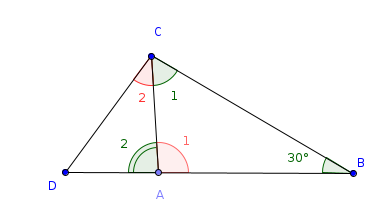
\includegraphics[scale = 0.35]{image_2}
		\begin{fourchoice}
				\choice{130}
				\choice{150}
				\choice{160}
				\choice{140}
		\end{fourchoice}
		}
		\question{%
		مقدار ساده شده عبارت
		$3(2x+a)-2(3a+x)$
		در کدام گزینه آمده است.
			\begin{fourchoice}[2]
				\choice{$-8x+9a$}
				\choice{$4x$}
				\choice{$8x-9a$}
				\choice{$-8x+9a$}
			\end{fourchoice}
		}
		\question{
			مساحت مستطیل به طول 
			$(2x+y)$
			و عرض
			$(2y+3x)$
			کدام است؟
			\begin{fourchoice}[2]
				\choice{$2(x^2+y^2+xy)$}
				\choice{$4(x^2-y^2+2xy)$}
   				\choice{$2(2x^2+y^2+3xy)$}
				\choice{$4(x^2+y^2+xy)$}
			\end{fourchoice}

		}
		\question{
			مقدار 
			x
			 در معادله 
			$\dfrac{1}{2}x-\dfrac{4}{5}=\dfrac{2}{3}x$
			کدام است.
			\begin{fourchoice}
				\choice{$-\dfrac{24}{5}$}
				\choice{$\dfrac{24}{5}$}
				\choice{$\dfrac{24}{35}$}
				\choice{$-\dfrac{24}{35}$}
			\end{fourchoice}

		}
		\question{
			اگر
			$3x-3=7x-2x+5$
			مقدار
			$x+4$
			کدام است؟
			\\

			\begin{fourchoice}
				\choice{-4}
				\choice{0}
				\choice{-1}
				\choice{+1}
			\end{fourchoice}
		}
		\question{
			پنج برابر عددی منهای ۳ مساوی با سه برابر همان عدد به اضافه ۷ است آن عدد را بیابید.
			\\
			\begin{fourchoice}
				\choice{5}
				\choice{10}
				\choice{2}
				\choice{$\frac{1}{2}$}
		\end{fourchoice}
		}
		\question{
			اگر
			$b=i, a = 2i-j$
			مختصات بردار 
			$\overrightarrow{x} $
			که به صورت 
			$\overrightarrow{x}=3a+4b $
			است، کدام است؟
			\\
			
			
			\begin{fourchoice}[2]
				\choice{$6i-3j$}
				\choice{$4i+3j$}
				\choice{$i+j$}
				\choice{$10i-3j$}
		\end{fourchoice}
		}
		\question{
بردار مختصاد یک رباط طوری طراحی شده است که از مبدأ مختصات یک واحد به راست و یک واحد به بالا حرکت می‌کند و یک مکث ی‌کند و همین روند را تکرار می‌کند. اگر این رباط در مکث ششم در نقطه $C$ باشد مقدار $5C+3j$ کدام است؟
\\
		\begin{fourchoice}
			\choice{$6i+6j$}
			\choice{$30j+23j$}
			\choice{$33i+30j$}
			\choice{$20i+23j$}
	\end{fourchoice}
		}
		\question{
مقدار $x$ را طوری بدست آورید که:
\\
$2x^2-2x(x+3) = 4+7(x+5)$
\\
		\begin{fourchoice}
			\choice{$-\frac{9}{13}$}
			\choice{$\frac{5}{13}$}
			\choice{$\frac{9}{1}$}
			\choice{$-\frac{6}{5}$}
	\end{fourchoice}
		}
		\question{
		اگر یک چند ضلعی منتظم از ۶ مثلث متساوی الاضلاع تشکیل شده باشد شکل حاصل چند ضلعی است و اندازه زاویه داخلی آن چند درجه است؟
		\\
		\begin{fourchoice}[2]
			\choice{8ضلعی و 135 درجه}
			\choice{6ضلعی و 120 درجه}
			\choice{4ضلعی و 90 درجه}
			\choice{5 ضلعی و 108 درجه}
			

		\end{fourchoice}


		}
		\question{
		در شکل زیر پاره خط
		$CD$
		را از روی خطر $BE$موازی خط
		$BA$
		رسم کرده‌ایم. اندازه زاویه $\widehat{ADC}$ را بدست آورید. 

		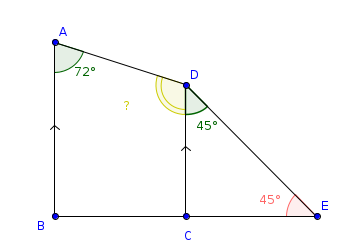
\includegraphics[scale = 0.35]{image_12}
		
		\begin{fourchoice}
			\choice{$\frac{153}{2}$}
			\choice{153}
			\choice{108}
			\choice{$\frac{108}{2}$}
		\end{fourchoice}
		}
		\question{
			مقدار
			$x-y$
			کدام است؟

			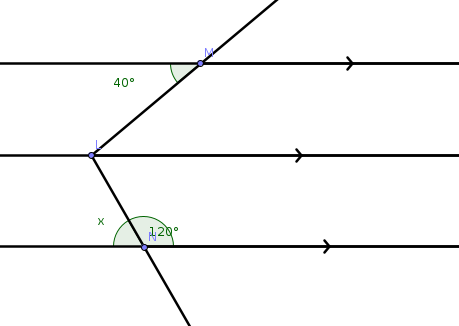
\includegraphics[scale = 0.35]{image_13}
			\\
			\begin{fourchoice}
				\choice{60}
				\choice{120}
				\choice{100}
				\choice{140}
			\end{fourchoice}
		}
			
		\question{
			در یک ۵ ضلعی منتظم مقدار یک زاویه خارجی برابر 
		$2x+10$
			است. مقدار$x$
			کدام است؟

			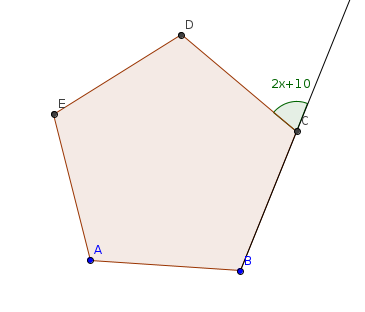
\includegraphics[scale = 0.35]{image_14}
			\\
			\begin{fourchoice}
				\choice{62}
				\choice{31}
				\choice{41}
				\choice{81}
			\end{fourchoice}
		}
	\end{questions}
\end{document}